
\documentclass[conference]{IEEEtran}

% --- Idioma y Codificación (Se cargan primero) ---
\usepackage[utf8]{inputenc}
\usepackage[spanish]{babel}

% --- Matemáticas, Formato y Estructuras Avanzadas ---
% Paquetes matemáticos y de formato avanzado agrupados:
\usepackage{amssymb, amsmath, amsthm, empheq, bm}
% Paquetes para estructuras enmarcadas y colores específicos:
\usepackage{mdframed, float}
\usepackage{color, colortbl, xcolor}
% --- Figuras, Tablas y Gráficos ---
% Paquetes para imágenes, tablas y gráficos agrupados:
\usepackage{graphicx, subcaption, caption, booktabs, multirow, psfrag}
\usepackage{pgfplots} % Se mantiene aparte para mejor visibilidad
% --- Hipervínculos y Documentación ---
\usepackage{hyperref, bookmark}

%%%%%%%%%%%%%%%%%%%%%%%%%%%%%%%%%%%%%%%%%%%%%%%%%%%%%%%%%%%%%%%%%%%%%%%%
% --- Paquete para Código Fuente ---}
% Paquete de colores (ya lo tienes, solo aseguramos que está antes de la config. de listings)


% --- Configuración de Estilo de MATLAB ---
%%%%%%%%%%%%%%%%%%%%%%%%%%%%%%%%%%%%%%%%%%%%%%%%%%%%%%%%%%%%%%%%%%%%%%%%
 % Para tablas con ancho de columna flexible
 % Para bloques de código
 % Para ajustar márgenes si es necesario
% --- AJUSTE CRÍTICO: La clase IEEEtran ya maneja los márgenes.
% **Se recomienda ENCARECIDAMENTE comentar o eliminar esta línea**
% para mantener el formato oficial de la conferencia.
% \usepackage{geometry}
% \geometry{a4paper, margin=1in}

%%%%%%%%%%%%%%%%%%%%%%%%%%%%%%%%%%%%%%%%%%%%%%%%%%%%%%%%%%%%%%%%%%%%%%%%%%%%%%%

% Other Settings

%%%%%%%%%%%%%%%%%%%%%%%%%% Define some useful colors %%%%%%%%%%%%%%%%%%%%%%%%%%
% Definición de colores (mantener separados para claridad en la configuración)
\definecolor{lightgreen}{HTML}{A9D18E}
\definecolor{lightred}{HTML}{F4C7C3}
\definecolor{ocre}{RGB}{243,102,25}
\definecolor{mygray}{RGB}{243,243,244}
\definecolor{deepGreen}{RGB}{26,111,0}
\definecolor{shallowGreen}{RGB}{235,255,255}
\definecolor{deepBlue}{RGB}{61,124,222}
\definecolor{shallowBlue}{RGB}{235,249,255}
%%%%%%%%%%%%%%%%%%%%%%%%%%%%%%%%%%%%%%%%%%%%%%%%%%%%%%%%%%%%%%%%%%%%%%%%%%%%%%%

%%%%%%%%%%%%%%%%%%%%%%%%%% Define an orangebox command %%%%%%%%%%%%%%%%%%%%%%%%
\newcommand\orangebox[1]{\fcolorbox{ocre}{mygray}{\hspace{1em}#1\hspace{1em}}}
%%%%%%%%%%%%%%%%%%%%%%%%%%%%%%%%%%%%%%%%%%%%%%%%%%%%%%%%%%%%%%%%%%%%%%%%%%%%%%%

%%%%%%%%%%%%%%%%%%%%%%%%%%%% Spanish Environments %%%%%%%%%%%%%%%%%%%%%%%%%%%%%
% Definición de estilos y entornos
\newtheoremstyle{mytheoremstyle}{3pt}{3pt}{\normalfont}{0cm}{\rmfamily\bfseries}{}{1em}{{\color{black}\thmname{#1}~\thmnumber{#2}}\thmnote{\,--\,#3}}
\newtheoremstyle{myproblemstyle}{3pt}{3pt}{\normalfont}{0cm}{\rmfamily\bfseries}{}{1em}{{\color{black}\thmname{#1}~\thmnumber{#2}}\thmnote{\,--\,#3}}
\theoremstyle{mytheoremstyle}
\newmdtheoremenv[linewidth=1pt,backgroundcolor=shallowGreen,linecolor=deepGreen,leftmargin=0pt,innerleftmargin=20pt,innerrightmargin=20pt,]{theorem}{Theorem}[section]
\theoremstyle{mytheoremstyle}
\newmdtheoremenv[linewidth=1pt,backgroundcolor=shallowBlue,linecolor=deepBlue,leftmargin=0pt,innerleftmargin=20pt,innerrightmargin=20pt,]{definition}{Definition}[section]
\theoremstyle{myproblemstyle}
\newmdtheoremenv[linecolor=black,leftmargin=0pt,innerleftmargin=10pt,innerrightmargin=10pt,]{problem}{Problem}[section]
%%%%%%%%%%%%%%%%%%%%%%%%%%%%%%%%%%%%%%%%%%%%%%%%%%%%%%%%%%%%%%%%%%%%%%%%%%%%%%%

%%%%%%%%%%%%%%%%%%%%%%%%%%%%%%% Plotting Settings %%%%%%%%%%%%%%%%%%%%%%%%%%%%%
\usepgfplotslibrary{colorbrewer}
\pgfplotsset{width=8cm,compat=1.9}
%%%%%%%%%%%%%%%%%%%%%%%%%%%%%%%%%%%%%%%%%%%%%%%%%%%%%%%%%%%%%%%%%%%%%%%%%%%%%%%

%%%%%%%%%%%%%%%%%%%%%%%%%%%%%%% Title & Author %%%%%%%%%%%%%%%%%%%%%%%%%%%%%%%%
\author{\IEEEauthorblockN{Jose David Hernández Rodriguez, Juan Andrés Díaz López, David Nicolas Ortega Peña,\\ Daniel Fernando Aranda Contreras}
\IEEEauthorblockA{Escuela E3T, Universidad Industrial de Santander\\
Correo electrónico: \{jose2221117, juan2205102, david2225138F1883, daniel2221648\}@correo.uis.edu.co}}
%%%%%%%%%%%%%%%%%%%%%%%%%%%%%%%%%%%%%%%%%%%%%%%%%%%%%%%%%%%%%%%%%%%%%%%%%%%%%%%

\begin{document}
    % Título
    \title{APLICACIÓN DEL CÓDIGO DE MEDIDA}
    \maketitle

    %\begin{abstract}
    
    %\end{abstract}

    \begin{IEEEkeywords}
        Código de Medida (CM), Incertidumbre de Medida, Transformadores de Medida, Burden, Clase de Exactitud, Generación Hidráulica, STN, SCADA, IOT, Modbus.
    \end{IEEEkeywords}

    \begin{abstract}
        La empresa ENERGER S.A. llevará a cabo la puesta en marcha de una planta generadora hidráulica de $\mathbf{975\ \text{MW}}$, que se compone de un grupo generador e instalaciones de operación (incluyendo servicios auxiliares). El grupo generador estará conformado por tres generadores síncronos monofásicos de $\mathbf{325\ \text{MVA}}$, $\mathbf{15\ \text{kV}}$, $\mathbf{60\ \text{Hz}}$ y $\mathbf{8}$ polos, el cual inyectará la potencia generada al STN a través de un transformador de $\mathbf{1000\ \text{MVA}}$, $\mathbf{15\ \text{kV}}/\mathbf{230\ \text{kV}}$ y conexión $\mathbf{\text{Dd}6}$. Las instalaciones de operación de la planta generadora operarán a $\mathbf{13.8\ \text{kV}}$ y serán alimentadas directamente desde el STN a través de un transformador de $\mathbf{500\ \text{kVA}}$, $\mathbf{230\ \text{kV}}/\mathbf{13.8\ \text{kV}}$ y conexión $\mathbf{\text{Dd}6}$.
    \end{abstract}

    \section{Introducción}
\begin{itemize}
  \item La planta generadora opera según tres regímenes (veasen en el cuadro \ref{tab:regimenes_operacion}) o intervalos, tanto en el grupo generador como en las instalaciones de operación.
  \item Debido a la disposición física de la planta generadora, la distancia entre los transformadores de medida correspondientes al grupo generador y el gabinete del sistema de medición es aproximadamente l1= 225 m; mientras esta distancia es aproximadamente l2 = 120 m entre los transformadores de medida correspondientes a las instalaciones de operación y el gabinete del sistema de medición.
  \item Con base en un análisis técnico-financiero, se definió que el esquema de medición deberá brindar la siguiente información: (i) energía generada (activa y no activa) por parte del grupo generador y (ii) energía consumida (activa y no activa) debida a las instalaciones para la operación del grupo generador.

\end{itemize}

\begin{table*}[t]
  \centering
  \caption{Regímenes de operación de la planta generadora.}
  \label{tab:regimenes_operacion}
  \begin{tabular}{ccccccc}
    \toprule
    \multirow{2}{*}{\textbf{Intervalo}} & \multicolumn{3}{c}{\textbf{Grupo generador}} & \multicolumn{3}{c}{\textbf{Instalaciones de operación}} \\
    \cmidrule(lr){2-4} \cmidrule(lr){5-7}
    & \textbf{Tiempo} & \textbf{Generación} & \textbf{fp} & \textbf{Tiempo} & \textbf{Consumo} & \textbf{fp} \\
    \midrule
    1 & 50\% & 85\% & 1.0 & 45\% & 85\% & 0.92 ad \\
    2 & 45\% & 80\% & 0.95 at & 50\% & 90\% & 0.95 ad \\
    3 & 5\% & 50\% & 0.91 at & 5\% & 70\% & 0.95 ad \\
    \bottomrule
  \end{tabular}
\end{table*}




\section{Tipos de frontera}
\begin{itemize}
  \item \textbf{Fronteras de generación:} Corresponde al punto de medición de una unidad o planta de generación donde las transferencias de energía equivalen a la energía neta entregada por el generador al STN, al STR o al SDL.
  \item \textbf{Fronteras de comercialización}: Punto de medición donde las transferencias de energía registradas permiten determinar la demanda de energía de un comercializador. A su vez, se clasifican en:
  \item \begin{itemize}
    \item \textbf{Fronteras de comercialización entre agentes:} Permite determinar la transferencia de energía entre mercados de comercialización o entre el STN y un mercado de comercialización.
    \item \textbf{Frontera de comercialización entre agentes y usuarios:}  Corresponde a toda frontera de comercialización que no cumple con los criterios de la frontera entre agentes. También incluye la frontera comercial de un usuario que se conecta directamente al STN.
  \end{itemize}
\end{itemize}


\section{Definición de los tipos de punto de medida}

Partiendo de la capacidad instalada por los generadores, y según la \textbf{tabla 1 del artículo 6 de la resolución CREG 038} se puede determinar que el tipo de punto de medición tanto para generaciones como para instalación de operación es \textbf{tipo 1}. Vease el cuadro \ref{tab:clasificacion_puntos_medicion}.


\begin{table*}[t]
  \centering
  \caption{Clasificación de puntos de medición.}
  \label{tab:clasificacion_puntos_medicion}
  \begin{tabular}{ccc}
    \toprule
    \textbf{Tipo de puntos de medición} & \textbf{Consumo o transferencia de energía, C [MWh-mes]} & \textbf{Capacidad Instalada, CI [MVA]} \\
    \midrule
    1 & $\ge 15.000$ \cellcolor{lightgreen} & $\ge 30$ \cellcolor{lightgreen} \\
    2 & $15.000 > C \ge 500$ & $30 > CI \ge 1$ \\
    3 & $500 > C \ge 50$ \cellcolor{lightred} & $1 > CI \ge 0,1$ \cellcolor{lightred} \\
    4 & $50 > C \ge 5$ & $0,1 > CI \ge 0,01$ \\
    5 & $C < 5$ & $CI < 0,01$ \\
    \bottomrule
  \end{tabular}
  \caption*{Tipos de puntos de medición.}
\end{table*}


En la tabla anterior (vease el cuadro \ref{tab:clasificacion_puntos_medicion}) está seleccionado con color verde el tipo de punto de medición para la frontera de generación y en color rojo el tipo de punto de medición para la frontera de comercialización. En este caso, como la frontera generación nos da un tipo más alto, este es el que se elige para ambas fronteras.

---
\section{Cantidad, tipo y clase de medidores y transformadores de medida requeridos de acuerdo con los tipos de frontera seleccionados}

Según lo establecido en la \textbf{resolución CREG 038 de 2014}, los tipos de frontera de generación y comercialización deben contar con un \textbf{medidor principal} y uno de \textbf{respaldo}. Además, el medidor de respaldo debe operar permanentemente y tener las mismas características técnicas que el medidor principal.

A continuación, se presenta la tabla para determinar la clase del medidor según su tipo de punto de medición:



\subsection{Medidores para la Frontera de Generación}
En la siguiente tabla (vease el cuadro \ref{tab:clase_medidor_generacion}) se presentan los medidores de potencia activa y reactiva según su clase. Es importante resaltar que estos medidores deben ser idénticos para que puedan entrar en funcionamiento.

\begin{table}[H]
    \centering
    \caption{Elección de la clase de medidor para la frontera de generación.}
    \label{tab:clase_medidor_generacion}
    \begin{tabular}{cccc}
        \toprule
        \textbf{MEDIDOR} & \textbf{CLASE} & \textbf{TRANSFORMADOR DE MEDIDA} & \textbf{CLASE} \\
        \midrule
        Activa & 0.2S & PT & 0.2 \\
        Reactiva & 2 & CT & 0.2S \\
        \bottomrule
    \end{tabular}
    \caption*{\textbf{Tabla 1.} Elección de la clase de medidor para la frontera de generación.}
\end{table}

\subsection{Medidores para la Frontera de Comercialización Entre Agente y Usuario}
En la siguiente tabla (vease el cuadro \ref{tab:clase_medidor_comercializacion}) se presentan los medidores de potencia activa y reactiva según su clase. Es importante resaltar que estos medidores deben ser idénticos para que puedan entrar en funcionamiento.

\begin{table}[H]
    \centering
    \caption{Elección de la clase de medidor para la frontera de comercialización.}
    \label{tab:clase_medidor_comercializacion}
    \begin{tabular}{cccc}
        \toprule
        \textbf{MEDIDOR} & \textbf{CLASE} & \textbf{TRANSFORMADOR DE MEDIDA} & \textbf{CLASE} \\
        \midrule
        Activa & 0.5S & PT & 0.5 \\
        Reactiva & 2 & CT & 0.5S \\
        \bottomrule
    \end{tabular}
    \caption*{\textbf{Tabla 2.} Elección de la clase de medidor para la frontera de comercialización.}
\end{table}

\subsection{Elección de Medidor Comercial para Frontera de Generación}

El medidor elegido que cumple con todos los requisitos técnicos para poder medir adecuadamente potencia activa y reactiva es el medidor \textbf{Acuvim-L}.

\begin{figure}[H]
    \centering
    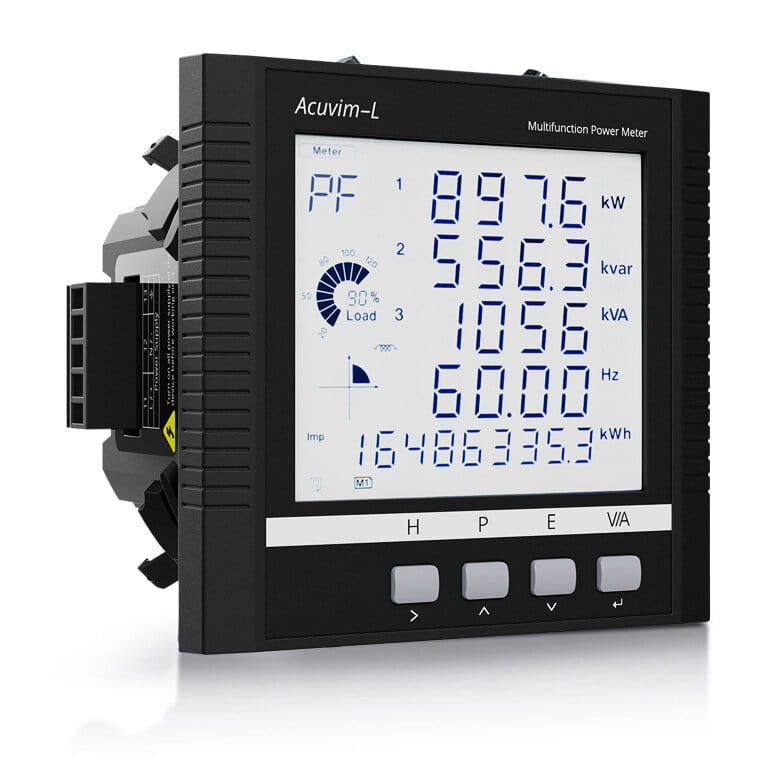
\includegraphics[width=0.8\columnwidth]{figs/medidor acuvin L.jpg} % Sustituir con la imagen real
    \caption{Medidor Acuvim-L}
    \label{fig:acuvim_l}
\end{figure}

\subsection{Elección de Medidor Comercial para Frontera de Comercialización}

El medidor elegido que cumple con todos los requisitos técnicos para poder medir adecuadamente potencia activa y reactiva es el medidor \textbf{Acuvim-EV300}.

\begin{figure}[H]
    \centering
    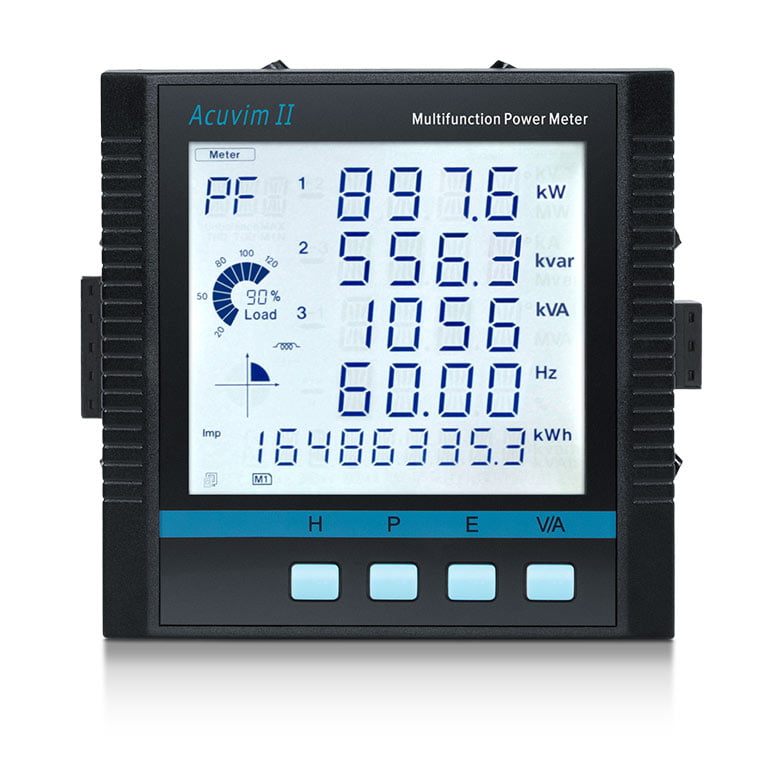
\includegraphics[width=0.8\columnwidth]{figs/Medidor acuvim-EV300.jpg} % Sustituir con la imagen real
    \caption{Medidor Acuvim-EV300}
    \label{fig:acuvim_ev300}
\end{figure}

---
\section{Esquema de conexión de los sistemas de medición}


En sistemas eléctricos de \textbf{230 kV}, la medición siempre se realiza de forma \textbf{indirecta}, utilizando transformadores de corriente (TC) y de tensión (TT), conforme a lo establecido en la Resolución CREG 038 de 2014.

\subsection{Medición Indirecta Simétrica}

Cuando la carga está \textbf{balanceada}, la conexión del medidor se clasifica como \textbf{indirecta simétrica}, ya que las magnitudes de corriente y tensión en cada fase se mantienen proporcionales y dentro de los límites de exactitud exigidos por la normativa, ver figura \ref{fig:esquema_simetrico}.


\subsection{Medición Indirecta Asimétrica}

Por el contrario, si la carga se encuentra \textbf{desbalanceada}, la conexión se considera \textbf{indirecta asimétrica}, debido a que las fases no presentan igualdad en magnitud ni en ángulo, generando registros de consumo diferentes entre ellas. ver figura \ref{fig:esquema_asimetrico} Esta situación es contemplada por la CREG como una condición que exige selección y verificación adecuada de los transformadores de medida para garantizar la confiabilidad de la medición.





---
\section{Selección de los transformadores de medición. Análisis de alternativas.}

\subsection{Frontera de generación}
Datos:
$S_{\text{generador}} = 975 \text{ [MVA]}$
$V_{\text{nom}} = 13.2 \text{ [kV]}$ (Nota: El texto usa $V_{\text{nom}} = 230 \text{ [kV]}$ para el cálculo, asumiendo el punto de medición)

Calculamos la corriente nominal. La fórmula se muestra a continuación:
\begin{equation}
    I_{\text{nom}} = \frac{S_{\text{generador}}}{\sqrt{3} \cdot V_{\text{nom}}} \text{ [A]}
\end{equation}
Sustituyendo valores para la medición en $230 \text{ kV}$:
\begin{align*}
    I_{\text{nom}} &= \frac{975 \text{ [MVA]}}{\sqrt{3} \cdot 230 \text{ [kV]}} \text{ [A]} \\
    I_{\text{nom}} &\approx 2447.46 \text{ [A]}
\end{align*}
Con esto, calculamos el $I_{p}'$.
\begin{equation}
    I_{p}' = C_T \cdot I_{\text{nom}} ; \quad C_T = 120\%
\end{equation}
\begin{align*}
    I_{p}' &= 120\% \cdot 2447.46 \\
    I_{p}' &\approx 2936.952 \text{ [A]}
\end{align*}
Luego, buscamos los valores más cercanos de corriente que soporte los CT y aproximamos nuestro valor hallado al valor comercial:
\begin{itemize}
    \item $R_{\text{TCT}} = 3000:5$
\end{itemize}
Ahora, calculamos el $R_{\text{TPT}}$:
\begin{equation}
    V_{\text{medidor}} = \frac{230 \text{ [kV]}}{120}
\end{equation}
\begin{align*}
    V_{\text{medidor}} &\approx 1916.66 \text{ [V]}
\end{align*}
Este valor se aproxima a un valor comercial:
\begin{itemize}
    \item $V_{\text{medidor}} \approx 2000 \text{ [V]}$
    \item $R_{\text{TPT}} = 2000:1$
\end{itemize}

\subsection{Frontera de consumo}
Datos:
$S_{\text{generador}} = 500 \text{ [kVA]}$
$V_{\text{nom}} = 13.8 \text{ [kV]}$

Calculamos la corriente nominal. La fórmula se muestra a continuación:
\begin{equation}
    I_{\text{nom}} = \frac{S_{\text{generador}}}{\sqrt{3} \cdot V_{\text{nom}}} \text{ [A]}
\end{equation}
Sustituyendo valores:
\begin{align*}
    I_{\text{nom}} &= \frac{500 \text{ [kVA]}}{\sqrt{3} \cdot 13.8 \text{ [kV]}} \text{ [A]} \\
    I_{\text{nom}} &\approx 20.91 \text{ [A]}
\end{align*}
Con esto, calculamos el $I_{p}'$:
\begin{equation}
    I_{p}' = C_T \cdot I_{\text{nom}} ; \quad C_T = 120\%
\end{equation}
\begin{align*}
    I_{p}' &= 120\% \cdot 20.91 \\
    I_{p}' &\approx 25.092 \text{ [A]}
\end{align*}
Luego, buscamos los valores más cercanos de corriente que soporte los CT y aproximamos nuestro valor hallado al valor comercial:
\begin{itemize}
    \item $R_{\text{TCT}} = 30:5$
\end{itemize}
Ahora, calculamos el $R_{\text{TPT}}$:
\begin{equation}
    V_{\text{medidor}} = \frac{13.8 \text{ [kV]}}{120}
\end{equation}
\begin{align*}
    V_{\text{medidor}} &\approx 115 \text{ [V]}
\end{align*}
Este valor se aproxima a un valor comercial:
\begin{itemize}
    \item $V_{\text{medidor}} \approx 115 \text{ [V]}$
    \item $R_{\text{TPT}} = 115:1$
\end{itemize}

---
\section{Análisis de la incertidumbre máxima que se presentará en la medición de las energías activa y de la potencia (energía) reactiva de acuerdo con el tipo de frontera comercial analizado}

\begin{itemize}
    \item Medidor de energía Activa 0.2S: 0.20 \%
    \item Medidor de energía Reactiva clase 2: 2.0 \%
    \item Transformador de Corriente CT clase 0.2S: 0.20 \%
    \item Transformador de Tensión clase 0.2S: 0.20\%
    \item Burden del CT: 0.16 \%
    \item E\% por cableado y conexiones: 0.10 \%
    \item E\% Fase Energía Reactiva: 0.03 \%
\end{itemize}
Para el tramo $225 \text{ m}$ con $50 \text{ mm}^2$, con $I_{\text{sec}}=4.895$ y $R_{\text{line}}=0.1552 \Omega$, se obtuvo un \textbf{burden} $\approx 3.72 \text{ VA}$.
Para el tramo $120 \text{ m}$ con $25 \text{ mm}^2$, con $V:0.81013$ y $R_{\text{line}}=0.1655 \Omega$, se obtuvo un \textbf{burden} $\approx 3.97 \text{ VA}$.

El CT está diseñado para $5 \text{ VA} \rightarrow 3.97/5=0.794$. El error aumenta proporcionalmente: $0.2\% \times 0.794 = 0.1588 \%$.

\begin{itemize}
    \item Suma directa de los \%: $0.86 \%$ (Peor de los casos, Activa)
    \item Suma de los RMS \%: $0.39 \%$ (Para Activa)
    \item Suma directa de los \%: $2.69 \%$ (se agrega el de fase y el medidor de reactiva)
    \item Suma de los RMS \%: $2.03 \%$ (Para Reactiva)
\end{itemize}
Para la frontera de \textbf{tipo 1}, compuesta por medidor principal y de respaldo \textbf{clase 0.2S} (energía activa), \textbf{clase 2} (energía reactiva), \textbf{CT 3000:5 clase 0.2S} y \textbf{PT clase 0.2}, se evaluó la incertidumbre total considerando los errores de cada elemento y el efecto del \textbf{burden} en los conductores secundarios.

Los cálculos se realizaron con longitudes de $225 \text{ m}$ ($50 \text{ mm}^2$) y $120 \text{ m}$ ($25-35 \text{ mm}^2$), obteniendo un \textbf{burden} aproximado de $\mathbf{3.72 \text{ VA}}$, valor inferior al nominal de los transformadores, por lo que no genera sobrecarga ni incrementa el error del sistema.

Combinando los errores de medidor, CT, PT y burden se obtiene:
\begin{itemize}
    \item Energía activa: \textbf{incertidumbre total} $\approx \mathbf{0.39 \%}$
    \item Energía reactiva: \textbf{incertidumbre total} $\approx \mathbf{2.03 \%}$
\end{itemize}
Estos valores cumplen con los límites establecidos por la \textbf{Resolución CREG 038 de 2014} para fronteras tipo 1. La principal contribución en la energía reactiva proviene del medidor clase 2, mientras que en la energía activa los errores se reparten entre los transformadores y el medidor.

---
\section{Análisis de las especificaciones del sistema de medición y su cumplimiento con las exigencias del código de medida con relación al Burden de los transformadores de medida y la caída de tensión que se presenta en los conductores del secundario de los transformadores de medida}

En este caso, el sistema de medición \textbf{cumple} con lo que pide la \textbf{Resolución CREG 038 de 2014}, ya que el \textbf{burden} total de los transformadores de medida se mantiene dentro de los valores permitidos.

Para las distancias de $225 \text{ m}$ y $120 \text{ m}$, con conductores de $50 \text{ mm}^2$ y $25-35 \text{ mm}^2$, la \textbf{caída de tensión} en el secundario del CT es de más o menos $\mathbf{0.7 \text{ a } 0.8 \text{ V}}$, lo que equivale a un \textbf{burden} cercano a $\mathbf{3.7 \text{ VA}}$.

Ese valor está \textbf{por debajo del nominal} ($\mathbf{5 \text{ VA}}$), así que los transformadores trabajan en su rango correcto y conservan la clase de exactitud ($\mathbf{0.2S}$ y $\mathbf{0.2}$).

En conclusión, el sistema de medición \textbf{cumple} con el \textbf{Código de Medida} tanto en el \textbf{burden} como en la \textbf{caída de tensión} de los secundarios.

%%%%%%%%%%%%%%%%%%%%%%%%%%%%%%%%%%%%%%%%%%%%%%%%%%%%%%%%%%




\begin{table*}[t]
  \centering
  \small % Reducimos la fuente para ayudar a que quepa en doble columna
  \caption{Requisitos de exactitud para medidores y transformadores de medida.}
  \label{tab:requisitos_exactitud}
  \begin{tabular}{ccccc}
    \toprule
    \textbf{T. punto de medicion} & \textbf{Índ. de clase activa} & \textbf{Índ de clase reactiva} & \textbf{Exactitud para CTs} & \textbf{Clase de exactitud para TPs} \\
    \midrule
    1 & 0,2 S & 2 & 0,2 S & 0,2 \\
    2 y 3 & 0,5 S & 2 & 0,5 S & 0,5 \\
    4 & 1 & 2 & 0,5 & 0,5 \\
    5 & 1 ó 2 & 2 ó 3 & -- & -- \\
    \bottomrule
  \end{tabular}
  \caption*{Tabla de requisitos de exactitud para medidores y transformadores de medida.}
\end{table*}

\subsubsection{Medidores para la Frontera de Generación}
En la siguiente Cuadro \ref{fig:esquema_asimetrico} se presentan los medidores de potencia activa y reactiva según su clase. Es importante resaltar que estos medidores deben ser idénticos para que puedan entrar en funcionamiento.

\subsubsection{Medidores para la Frontera de Comercialización Entre Agente y Usuario}
En la siguiente tabla se presentan los medidores de potencia activa y reactiva según su clase. Es importante resaltar que estos medidores deben ser idénticos para que puedan entrar en funcionamiento.





\begin{figure*}[t]
    \centering
    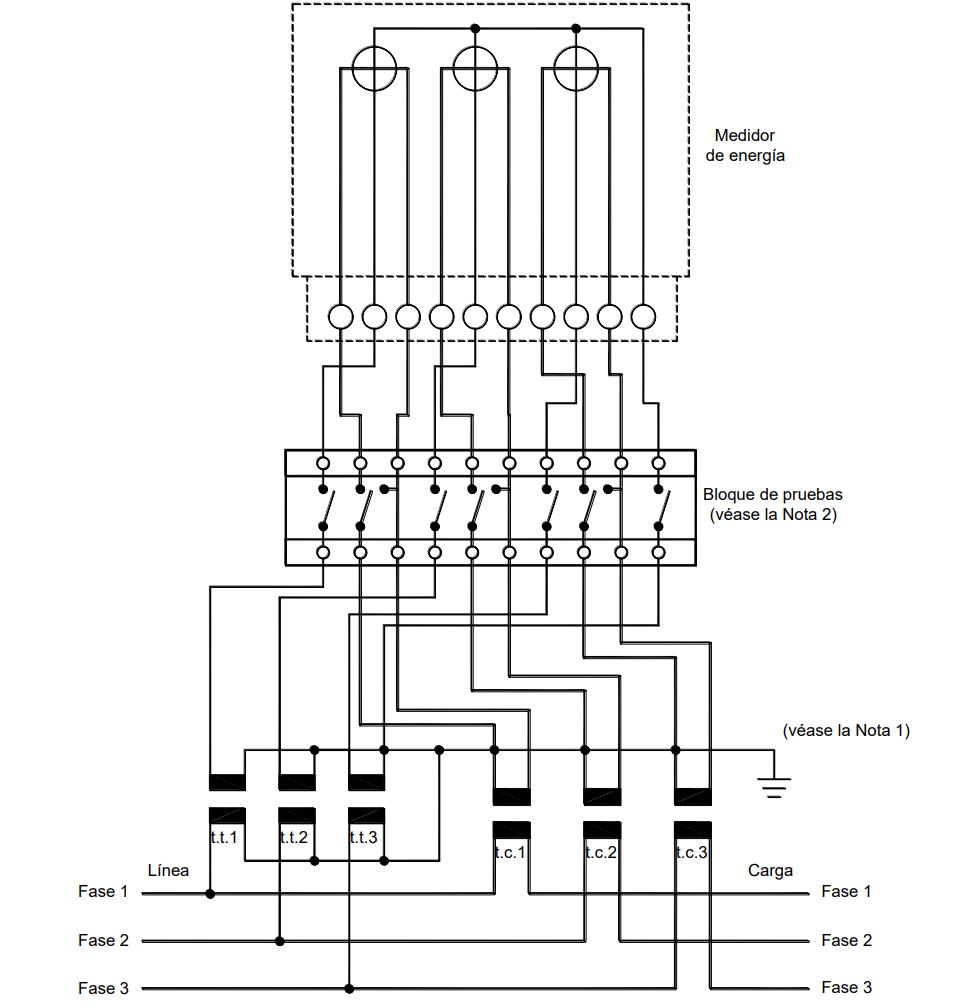
\includegraphics[width=\columnwidth]{figs/figura_esquema_simetrico.png}
    \caption{Esquema de conexiones medidor trifásico tetrafilar para medición indirecta entre tres elementos, conexión simétrica.}
    \label{fig:esquema_simetrico}
\end{figure*}

Por el contrario, si la carga se encuentra \textbf{desbalanceada}, la conexión se considera \textbf{indirecta asimétrica}, debido a que las fases no presentan igualdad en magnitud ni en ángulo, generando registros de consumo diferentes entre ellas. Esta situación es contemplada por la CREG como una condición que exige selección y verificación adecuada de los transformadores de medida para garantizar la confiabilidad de la medición.

\begin{figure*}[t]
    \centering
    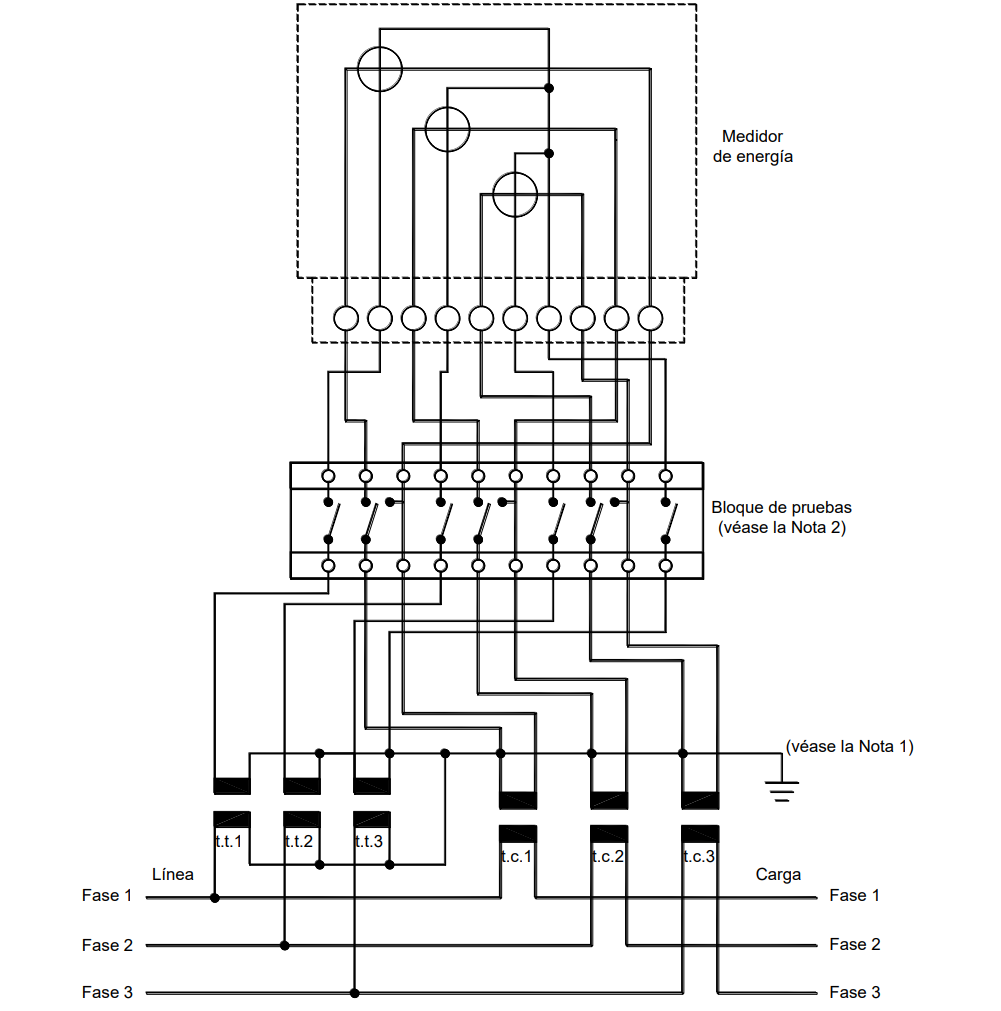
\includegraphics[width=\columnwidth]{figs/figura_esquema_asimetrico.png}
    \caption{Esquema de conexiones medidor trifásico tetrafilar para medición indirecta en tres elementos, conexión asimétrica.}
    \label{fig:esquema_asimetrico}
\end{figure*}



\section*{Ecuaciones Clave de Burden de Transformadores de Medida}

\subsection*{Para el Transformador de Corriente (TC)}

Las ecuaciones de carga (Burden) para el TC se centran en las pérdidas por corriente ($I^2 \cdot R$) en el cableado y la suma de la carga de los medidores.

\begin{align*}
    R_{\text{cableado}} &= r \cdot (2 \cdot L) \\
    S_{VA, \text{cableado}} &= I_{\text{sec}}^{2} \cdot R_{\text{cableado}} \\
    VA_{\text{TC, Total}} &= S_{VA, \text{cableado}} + 2 \cdot \text{Burden}_{\text{medidor}}
\end{align*}

\vspace{0.5cm}

\subsection*{Para el Transformador de Tensión (TT)}

La ecuación de carga (Burden) para el TT se calcula usando la tensión de fase ($V_{\text{fase}} = V_{\text{med}} / \sqrt{3}$) y la resistencia total en serie ($R_{\text{serie}}$).

\begin{equation}
    VA_{\text{medidor}} = \frac{V_{\text{fase}}^{2}}{R_{\text{conductor}} + R_{\text{medidor}}} = \frac{\left(\frac{V_{\text{med}}}{\sqrt{3}}\right)^2}{R_{\text{conductor}} + R_{\text{medidor}}}
\end{equation}

Donde la Carga Total (Burden) del TT es:
$$ VA_{\text{TT, Total}} = VA_{\text{medidor}} + VA_{\text{conductor}} $$

\begin{align*}
    \text{Condición de Adecuación} &: \left( \text{Burden}_{\text{TC, Nominal}} > VA_{\text{TC, Total}} \right) \quad \text{Y} \\ \quad \left( VA_{\text{TC, Total}} > 0.25 \cdot \text{Burden}_{\text{TC, Nominal}} \right)
\end{align*}


\section{Análisis de Incertidumbre en Medición de Energía Activa y Reactiva (TC y TT)}
Para el análisis se esta considerando un medidor de respaldo ademas de un cable AWG 14, en donde $r_{AC}=10.17[\Omega/km]$ a una temperatura de 75 °C. y por la cantidad de distancia el medidor con un valor nominal de corriente de 1 [A].
El código MATLAB realiza el cálculo del \textbf{Burden (Carga Aparente) Total} ($\text{VA}_{\text{real}}$) para los Transformadores de Corriente (TC) y los Transformadores de Tensión (TT), evaluando su idoneidad frente a los burdens nominales o comerciales ($\text{VA}_{\text{nominal}}$).

La \textbf{incertidumbre máxima} en la medición de energías se presenta cuando el transformador opera \textbf{fuera de su rango de precisión} garantizado, es decir, cuando la condición de cumplimiento ($\text{CUMPLE}$) no se satisface ($\text{NO CUMPLE}$).-

\subsection{Criterios de Cumplimiento y Precisión}

\begin{itemize}
    \item \textbf{TC (Transformador de Corriente):} La precisión se garantiza si la carga real está entre el 25\% y el 100\% del nominal:
    $$\frac{1}{4} \cdot \text{VA}_{\text{nominal}} < \text{VA}_{\text{real}} < \text{VA}_{\text{nominal}}$$
    \item \textbf{TT (Transformador de Tensión):} La precisión se garantiza si la carga real es mayor a cero y menor que el nominal:
    $$0 < \text{VA}_{\text{real}} < \text{VA}_{\text{nominal}}$$
\end{itemize}

\subsection{Modelo del calculo}
\subsubsection{Para el caso del TC}
% Longitud Total (km)

\begin{equation*}
l \, [\text{km}] = 2 \cdot \frac{L_{\text{met}} \, [\text{m}]}{1000 \, [\frac{\text{m}}{\text{km}}]}
\end{equation*}

% Resistencia Total [\Omega]
\begin{equation*}
R \, [\Omega] = r \, [\frac{\Omega}{\text{km}}] \cdot l \, [\text{km}]
\end{equation*}

% Potencia Aparente del Cableado [VA]
\begin{equation*}
S_{\text{VA}} \, [\text{VA}] = I^2 \, [\text{A}^2] \cdot R \, [\Omega]
\end{equation*}

% Carga Total del TC (Burden) [VA]
\begin{equation*}
\text{VA}_{\text{tc}} \, [\text{VA}] = S_{\text{VA}} \, [\text{VA}] + 2 \cdot \text{Burden}_{\text{med}} \, [\text{VA}]
\end{equation*}

% Condición de Cumplimiento (Precisión 25\% - 100\%)
\begin{equation*}
\text{Burden}_{C} \, [\text{VA}] \cdot 0.25 < \text{VA}_{\text{tc}} \, [\text{VA}] < \text{Burden}_{C} \, [\text{VA}]
\end{equation*}

\subsubsection{Para el caso del TT}
% Resistencia del Medidor [\Omega] - Dos medidores en paralelo
\begin{equation*}
R_{\text{medidor}} \, [\Omega] = \frac{R_A \, [\Omega] \cdot R_B \, [\Omega]}{R_A \, [\Omega] + R_B \, [\Omega]}
\end{equation*}

% Resistencia Total Serie [\Omega]
\begin{equation*}
R_{\text{serie}} \, [\Omega] = R_{\text{conductor}} \, [\Omega] + R_{\text{medidor}} \, [\Omega]
\end{equation*}

% Corriente del Conductor [A]
\begin{equation*}
I_{\text{conductor}} \, [\text{A}] = \frac{\left(\frac{V_{\text{med}} \, [\text{V}]}{\sqrt{3}}\right)}{\sqrt{R_{\text{serie}} \, [\Omega]}}
\end{equation*}

% Potencia Aparente del Medidor [VA]
\begin{equation*}
\text{VA}_{\text{medidor}} \, [\text{VA}] = \frac{\left(\frac{V_{\text{med}} \, [\text{V}]}{\sqrt{3}}\right)^2}{R_{\text{serie}} \, [\Omega]}
\end{equation*}

% Potencia Aparente del Conductor [VA]
\begin{equation*}
\text{VA}_{\text{conductor}} \, [\text{VA}] = I_{\text{conductor}}^2 \, [\text{A}^2] \cdot R_{\text{conductor}} \, [\Omega]
\end{equation*}

% Carga Total del TT (Burden) [VA]
\begin{equation*}
\text{VA}_{\text{tt}} \, [\text{VA}] = \text{VA}_{\text{medidor}} \, [\text{VA}] + \text{VA}_{\text{conductor}} \, [\text{VA}]
\end{equation*}

% Condición de Cumplimiento (Precisión 0\% - 100\%)
\begin{equation*}
0 < \text{VA}_{\text{tt}} \, [\text{VA}] < \text{Burden}_{C} \, [\text{VA}]
\end{equation*}
\subsubsection{Datasheet de los medidores seleccionados}
\begin{figure}[H]
    \centering
    \includegraphics[width=0.8\columnwidth]{figs/Acuvim L F.generación.png} % Sustituir con la imagen real
    \caption{Medidor en el lado de BT en generación.}
    \label{fig:BT_gen}
\end{figure}
\begin{figure}[H]
    \centering
    \includegraphics[width=0.8\columnwidth]{figs/Acuvim L F.generación.png} % Sustituir con la imagen real
    \caption{Medidor en el lado de BT en las instalaciones de operación.}
    \label{fig:BT_carga}
\end{figure}



\begin{figure}[H]
    \centering
    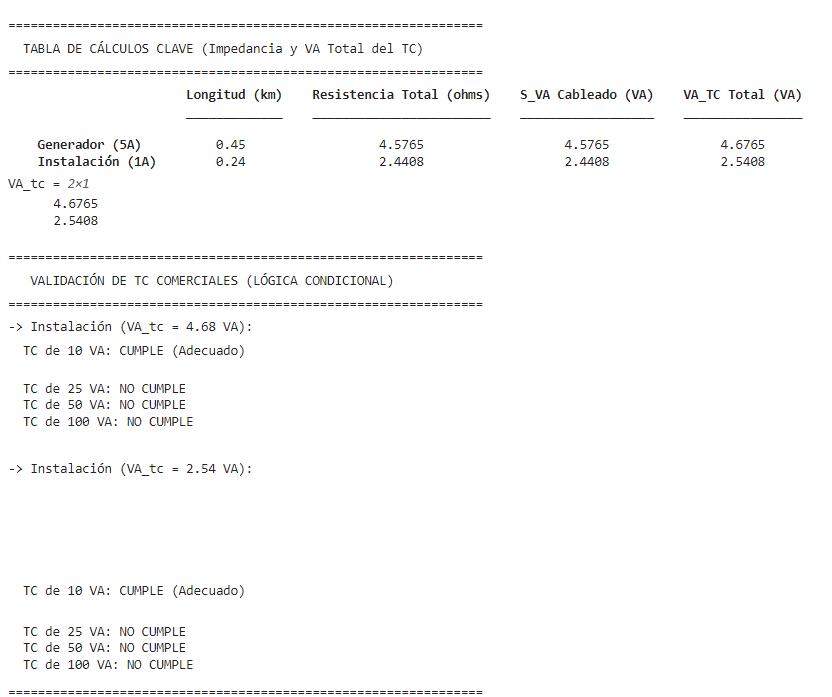
\includegraphics[width=0.8\columnwidth]{figs/6 TC.png} % Sustituir con la imagen real
    \caption{resultados del análisis de burden para el Transformador de Tensión (TC) para el generador y instalaciones de operación.}
    \label{fig:TC}
\end{figure}


\subsection{resultados del Análisis de Burden}
\begin{figure}[H]
    \centering
    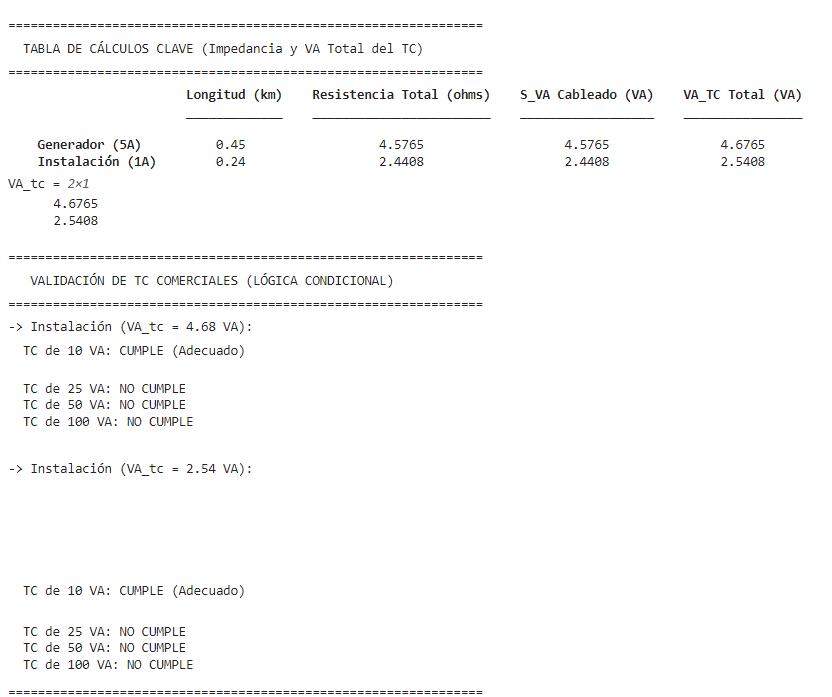
\includegraphics[width=0.8\columnwidth]{figs/6 TC.png} % Sustituir con la imagen real
    \caption{resultados del análisis de burden para el Transformador de Tensión (TC) para el generador y instalaciones de operación.}
    \label{fig:TC}
\end{figure}

\begin{figure}[H]
    \centering
    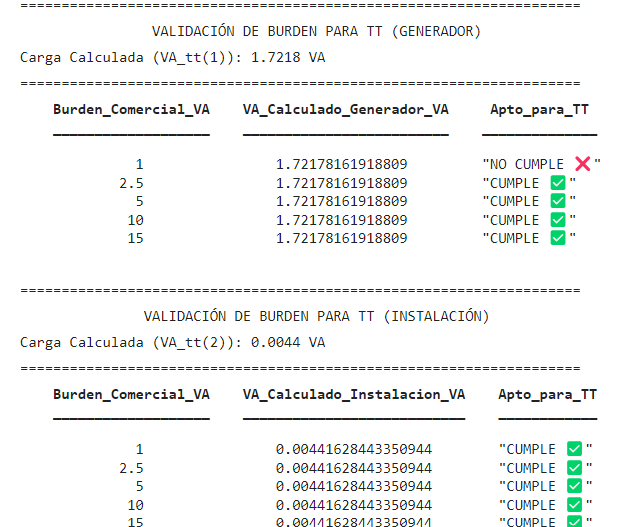
\includegraphics[width=0.8\columnwidth]{figs/6 TT.png} % Sustituir con la imagen real
    \caption{resultados del análisis de burden para el Transformador de Tensión (TT) para el generador y instalaciones de operación.}
    \label{fig:TT}
\end{figure}


    \nocite{*} % Asegura que todas las entradas de la bibliografía se incluyan, incluso si no se citan directamente
    \bibliographystyle{IEEEtran}
    \bibliography{ref} % Asegúrate de que tu archivo de bibliografía se llama 'ref.bib'

\end{document}